%% The first command in your LaTeX source must be the \documentclass command.
%%
%% Options:
%% twocolumn : Two column layout. Do not use twocolumn for papers submitted to CEUR-WS!
%% hf: enable header and footer.
\documentclass[
% twocolumn,
% hf,
]{ceurart}

%%
%% One can fix some overfulls
\sloppy

%%
%% Minted listings support 
%% Need pygment <http://pygments.org/> <http://pypi.python.org/pypi/Pygments>
\usepackage{listings}
\usepackage{graphicx}
\usepackage{multirow}
\usepackage{tikz}
\usetikzlibrary{arrows.meta, positioning, shapes.geometric}
%% auto break lines
\lstset{breaklines=true}

%%
%% end of the preamble, start of the body of the document source.
\begin{document}

%%
%% Rights management information.
%% CC-BY is default license.
\copyrightyear{2026}
\copyrightclause{Copyright for this paper by its authors.
  Use permitted under Creative Commons License Attribution 4.0
  International (CC BY 4.0).}

%%
%% This command is for the conference information
\conference{CLEF'26}

%%
%% The "title" command
\title{CheckMate at CheckThat! 2026: Fusion-Based Retrieval, Reasoning-Trace Ranking, and Citation-Controlled Article Generation}

% \tnotemark[1]
% \tnotetext[1]{You can use this document as the template for preparing your
%   publication. We recommend using the latest version of the ceurart style.}

%%
%% The "author" command and its associated commands are used to define
%% the authors and their affiliations.

\author[1]{Taha Munawar}[%
% orcid=0000-0001-7116-9338,
email=tm08122@st.habib.edu.pk,
]
\cormark[1]
\address[1]{Dhanani School of Science and Engineering, Habib University, Karachi, Pakistan}

\author[1]{Abdullah Amir}[%
email=aa08453@st.habib.edu.pk,
]

\author[1]{Faisal Alvi}[%
email=faisal.alvi@sse.habib.edu.pk,
]

\author[1]{Abdul Samad}[%
email=abdul.samad@sse.habib.edu.pk,
]

\cortext[1]{Corresponding author.}

\begin{abstract}
  This paper describes our participation as team \textit{CheckMate} in the CheckThat! 2026 Lab. We address three tasks covering different parts of the automated fact-checking pipeline: source retrieval for scientific web claims, fact-checking numerical claims through reasoning-trace ranking, and full fact-checking article generation. For Task 1, we develop a multilingual retrieval and reranking pipeline based on Qwen3 dense retrieval, listwise reranking, and calibrated score fusion. For Task 2, we explore pointwise, pairwise, and preference-based ranking methods for selecting useful reasoning traces for numerical claim verification. For Task 3, we build a staged article-generation pipeline that filters noisy evidence, extracts claim-aware evidence snippets, constructs verdict-aware evidence packets, and generates citation-controlled fact-checking articles. On the official evaluation phase, our Task 1 system achieved 0.7194 average MRR@5, our Task 2 Arabic and Spanish submissions achieved average scores of 0.5599 and 0.4093 respectively, and our Task 3 system achieved a mean score of 0.328.
\end{abstract}

%%
%% Keywords. The author(s) should pick words that accurately describe
%% the work being presented. Separate the keywords with commas.
% \begin{keywords}
  % LaTeX class \sep
  % paper template \sep
  % paper formatting \sep
  % CEUR-WS
% \end{keywords}

%%
%% This command processes the author and affiliation and title
%% information and builds the first part of the formatted document.
\maketitle

\section{Introduction}
The rapid proliferation of misinformation across multilingual social media platforms necessitates the development of robust, automated systems capable of verifying complex claims at scale. While early fact-checking research focused primarily on simple, ``flat'' claim-to-document matching, the current consumer landscape requires the generation of transparent, long-form explanations. To address these challenges, the CLEF 2026 CheckThat! Lab introduces three interconnected tasks, all of which we attempt in this work \cite{10.1007/978-3-032-21321-1_43}.

Task 1 involves grounding informal discourse of scientific claims made by multilingual social media posts (in English, German, and French) that implicitly cite a ``recent study'' or a ``university report'' without providing any direct links. It requires formal evidence by verifying these claims from a candidate pool of scientific papers. 

Task 2 shifts the focus from simple classification to test-time scaling and reasoning quality. Given a claim in English, Spanish, or Arabic, participants must rank multiple LLM-generated reasoning traces based on their utility and logical soundness. By introducing a re-ranking framework for reasoning paths, this task aims to mitigate ``reasoning drift'' in Large Language Models (LLMs), ensuring that the final verdict is not just correct but also derived from a valid rationalization of quantitative evidence.

Task 3 introduces a generative challenge that requires synthesizing a claim, its veracity, and a set of evidence documents into a cohesive, professional fact-checking article, moving beyond short-form justification toward full-scale automation of the journalistic process.

To facilitate reproducibility, our code, exact prompts, and hyperparameter configurations are publicly available at \url{https://github.com/tahamunawar/LLM-CheckThat2026}.

\section{Related Work}

\subsection{Task 1: Source Retrieval for Scientific Web Claims}

Scientific claim-source retrieval requires matching informal social media claims to formal academic publications, creating both a stylistic and semantic gap between queries and evidence documents. Prior CheckThat! work on related claim-to-source tasks showed that multi-stage pipelines are effective for this setting, typically using an initial retrieval stage followed by neural reranking \cite{hafid2025overview}. Earlier systems also demonstrated the value of combining lexical or dense retrieval with rerankers, using hard negatives to improve robustness against superficial keyword overlap \cite{staudinger2025atom, sager2025deep, thapliyal2025scire, ashbaugh2025airwaves}. These findings directly motivate our Task 1 design: a multilingual dense retriever for candidate generation, listwise reranking over retrieved candidates, and calibrated fusion between complementary ranking signals. The multilingual setting also requires cross-lingual alignment between informal claims and scientific article representations.

\subsection{Task 2: Fact-Checking Numerical Claims}

Numerical claim verification is challenging because models must reason over quantities, dates, temporal scopes, and sometimes conflicting evidence. Prior work on numerical fact-checking benchmarks such as QuanTemp and QuanTemp++ highlights that quantitative claims require more than surface-level textual matching \cite{quantemp, quantempplus}. In LLM-based verification, a further challenge is reasoning drift, where a model begins with a plausible reasoning path but reaches an unsupported verdict after misinterpreting numerical or temporal evidence \cite{verifierfc}. Test-time scaling methods address this by generating multiple candidate reasoning traces, but this shifts the problem toward selecting the most reliable trace. This motivates verifier and reward-model approaches that evaluate reasoning quality rather than only the final answer \cite{lightman2023prm, setlur2024prm}. Our Task 2 methods follow this direction by comparing pointwise scoring, pairwise ranking, order-debiased pairwise prompting, PREPAIR-style structured comparison, and DPO with Bradley-Terry reward modeling for ranking reasoning traces.

\subsection{Task 3: Generating Full Fact-Checking Articles}

Automated fact-checking has increasingly moved beyond verdict prediction toward generating explanations and full fact-checking articles. Earlier explanation-generation work argued that fact-checking systems should justify their predictions, not merely classify claims \cite{atanasova2020generating}. More recent article-generation frameworks such as QRAFT frame fact-checking article writing as a dedicated generation task that resembles the workflow of professional fact-checkers \cite{sahnan2026qraft}. However, generated explanations and articles can suffer from weak evidence attribution, hallucinated support, and inaccurate citation use, making evidence selection and attribution central to trustworthy generation \cite{xing2025evidence}. These concerns motivate our Task 3 pipeline, which separates source usability triage, claim-aware evidence extraction, verdict-aware evidence packet construction, and final article generation. Unlike direct generation from all retrieved sources, our approach restricts the generator to selected evidence identifiers and inserts citations deterministically, reducing the risk of invented or malformed source links.

\section{Datasets}

\subsection{Task 1: Source Retrieval for Scientific Web Claims}

Task 1 uses the official multilingual claim-source retrieval dataset, where English, French, and German social-media claims are mapped to gold scientific articles from a 10,000-document collection \cite{clef-checkthat:2026:task1}. Table~\ref{tab:task1_datasets} summarizes the split sizes.

\begin{table}[h]
\caption{Task 1 query dataset distribution.}
\label{tab:task1_datasets}
\centering
\begin{tabular}{lccc}
\toprule
Language & Train & Dev & Test \\
\midrule
English & 14,977 & 3,905 & 6,080 \\
French  & 2,807  & 702   & 1,220 \\
German  & 1,460  & 386   & 876 \\
\midrule
Total   & 19,244 & 4,993 & 8,176 \\
\bottomrule
\end{tabular}
\end{table}

\subsection{Task 2: Fact-Checking Numerical Claims}

Task 2 consists of numerical fact-checking claims in English, Spanish, and Arabic \cite{clef-checkthat:2026:task2}. For each claim, the dataset provides 20 LLM-generated reasoning traces that must be ranked according to their usefulness for verification. The English split is based on QuanTemp, while the Spanish and Arabic splits are adapted from previous CheckThat! numerical claim verification data. 

\begin{table}[h]
\caption{Task 2 dataset statistics.}
\label{tab:task2_stats}
\centering
\begin{tabular}{lc}
\toprule
Language & Claims \\
\midrule
English & 8,000 \\
Spanish & 2,808 \\
Arabic & 3,260 \\
\bottomrule
\end{tabular}
\end{table}

\subsection{Task 3: Generating Full Fact-Checking Articles}

Task 3 uses the WatClaimCheck dataset for full fact-checking article generation \cite{clef-checkthat:2026:task3}. Each example provides a claim, its veracity label, and a set of evidence documents. For our final run, we used the official test split, containing 1,158 claims and 8,979 total evidence source references, with an average of 7.75 sources per claim.

\section{System Description}

\subsection{Task 1: Source Retrieval for Scientific Web Claims}

Task 1 was approached as a multi-stage retrieval and reranking problem. Given a multilingual scientific web claim in English, French, or German, the goal was to retrieve the correct source or best-evidence publication from a collection of 10,000 scientific articles. Our final system evolved through several stages: an initial multilingual dense retriever, a stronger Qwen-based retriever, listwise neural reranking, and finally calibrated multi-model fusion.

\subsubsection{Early Dense Retrieval Baseline}

Our initial system used \texttt{intfloat/multilingual-e5-large} as a dense dual-encoder retriever. Scientific documents were represented using structured metadata strings containing title, abstract, venue, and author fields. We also experimented with chunked tokenization, where long document representations were split into overlapping 510-token chunks. To make training more robust, we mined hard negatives: incorrect papers with high lexical overlap with the claim. These hard negatives acted as ``trick papers'', forcing the model to distinguish true source relevance from superficial vocabulary overlap. The retriever was trained using Multiple Negatives Ranking Loss.

\subsubsection{Retriever Replacement with Qwen3-Embedding-8B}

To address the retriever bottleneck, we replaced the e5 baseline with Qwen3-Embedding-8B and fine-tuned it using LoRA. Queries were formatted using an instruction prompt describing the task, while documents were represented using title and abstract text. The model was trained using Cached Multiple Negatives Ranking Loss, with an effective batch size of 128.

This retriever substantially improved Stage 1 performance. The multilingual-e5-large baseline achieved 0.6282 MRR@5, while the Qwen3-Embedding-8B LoRA retriever reached approximately 0.6793 MRR@5. This confirmed that better candidate generation was essential for the rest of the pipeline.

\subsubsection{Listwise Reranking over Qwen Candidates}

After improving the retriever, we used the Qwen3-Embedding-8B LoRA model to generate top-10 candidate sets for each query. These candidates were then used to train listwise rerankers. Each training group contained one gold document and nine hard negatives retrieved by the Qwen retriever. The reranker was trained with a listwise softmax cross-entropy loss.

We tested multiple rerankers. A listwise \texttt{BAAI/bge-reranker-v2-m3} reranker improved performance to 0.7094 MRR@5 after fusion with dense retrieval scores. This first alpha-fusion experiment showed that the retriever and reranker were complementary, since pure retrieval and pure reranking were both weaker than their weighted combination. Therefore, later reranker experiments retained fusion as a core part of the pipeline. We then trained \texttt{Qwen/Qwen3-Reranker-8B} using LoRA. This model scored each query--document pair using a yes/no relevance prompt, where the final relevance score was computed as the difference between the ``yes'' and ``no'' logits. Due to high compute cost, the Qwen3-Reranker-8B model was trained for one epoch only, but it still achieved 0.7400 MRR@5 as a pure reranker and 0.7435 MRR@5 after fusion with the dense retriever.

We also tested \texttt{nvidia/Llama-nemotron-rerank-1b-v2}. Although Nemotron was weaker than Qwen3-Reranker-8B on its own, it provided complementary ranking behavior. The Nemotron reranker achieved 0.7179 MRR@5 as a pure reranker and 0.7284 MRR@5 after fusion with the Qwen dense retriever.

\subsubsection{Final Multi-Model Fusion}

The final system combines three complementary signals: the Qwen3-Embedding-8B dense retriever score, the Qwen3-Reranker-8B score, and the Nemotron reranker score. Since these models produce scores on different scales, direct score addition is not ideal. Prior retrieve-and-rerank work has used softmax-normalized retriever and reranker scores as comparable passage-level distributions, motivating our use of query-level score normalization before fusion \cite{glass-etal-2022-re2g}. We therefore used temperature-scaled softmax/log-probability fusion, where each model's scores are first normalized at the query level over the top-10 candidates:

\[
s = w_d \log \mathrm{softmax}(s_d/T_d) +
    w_q \log \mathrm{softmax}(s_q/T_q) +
    w_n \log \mathrm{softmax}(s_n/T_n).
\]

Here, $s_d$, $s_q$, and $s_n$ denote the dense retriever, Qwen reranker, and Nemotron scores.

\subsection{Task 2: Fact-Checking Numerical Claims}
We explored two directions: parameter scaling and relational trace ranking. The relational methods compare traces directly using pairwise prompting, PREPAIR-style scorecards, and DPO with Bradley--Terry reward modeling.

\subsubsection{Baseline Approach}
The baseline utilizes a Llama 3.2 1B Instruct model in a point-wise ranking configuration. In this setup, the model processes a single reasoning trace in isolation for each claim. 

\subsubsection{Parameter Scaling}
The first optimization phase explores the impact of model scale by swapping the 1B baseline for the more sophisticated Llama 3.2 3B Instruct model. The model is loaded using 4-bit quantization. This phase tests the hypothesis that the superior reasoning capabilities of the 3B model can overcome the logical errors observed in the 1B baseline, even when compressed, while keeping the same point-wise architecture intact.

\subsubsection{Pairwise Ranking - Round Robin Tournament}

The second approach implements a Pairwise Cross-Encoder \cite{lee2025evaluating} using the base Llama 3.2 1B model. By processing pairs of candidate traces simultaneously, the model leverages self-attention for direct relational reasoning. Traces compete in a Round-Robin tournament, accumulating points to yield a normalized win-score. During inference, these scores aggregate into a Best-of-N (BoN) selection to determine the final veracity verdict. Keeping the base model constant isolates the methodology's specific impact on ranking accuracy and class bias.

\subsubsection{Pairwise Ranking - Elimination Tournament}
To overcome compute limitations, an elimination bracket replaces the round-robin tournament. Traces are paired based on their BM25 seed scores to prevent top-tier, well-reasoned traces from eliminating each other early on. The final five remaining traces are designated as the top five by rank.

\subsubsection{Pairwise Ranking Prompting}
Adapted from Pairwise Ranking Prompting (PRP) \cite{prp}, every pair is evaluated bidirectionally, both ($A$ vs. $B$) and ($B$ vs. $A$), to eliminate positional bias. Averaging the logit outputs from both directions yields a final win-margin, ensuring rankings reflect logical merit rather than document order.

\subsubsection{PREPAIR}
PREPAIR \cite{PrePAIR} attempts to mitigate context collapse by first extracting independent, unbiased insights from each trace to create a pointwise scorecard. This scorecard acts as a structured rationale behind the model's attention to specific logical flaws or numerical certainties. These are aggregated for final pairwise comparison, thus balancing absolute and relational logic, as well as mitigating the greater time complexity issue with naive pairwise ranking. 

\subsubsection{DPO \& Bradley-Terry Reward Modeling}

To bridge pairwise accuracy and pointwise speed, we converted pairwise trace preferences into
preferred--rejected training examples. Instead of performing all pairwise comparisons at inference
time, we used DPO-style preference optimization to train the model to assign higher scores to traces
that were preferred during pairwise comparison.

The Bradley-Terry model maps a trace's latent quality to an unobserved reward value $r$. The probability that trace $i$ is preferred over trace $j$ ($i \succ j$) is defined as:

\begin{equation}
P(i \succ j) = \sigma(r_i - r_j) = \frac{1}{1 + e^{-(r_i - r_j)}}
\end{equation}

The reward model is trained by minimizing the negative log-likelihood of these preferences over a dataset $D$:

\begin{equation}
\mathcal{L}(\theta) = -\mathbb{E}_{(x, y_w, y_l) \sim D} \left[ \log \sigma \left( r_\theta(x, y_w) - r_\theta(x, y_l) \right) \right]
\end{equation}

where $x$ is the context, and $y_w$ and $y_l$ are the preferred and rejected completions, respectively.

\subsection{Task 3: Generating Full Fact-Checking Articles}

The core rationale behind our staged architecture was to strictly constrain the generative model. Because end-to-end LLMs frequently hallucinate source URLs and conflate evidence, separating evidence extraction from generation allowed us to enforce deterministic, programmatically controlled citations.

For Task 3, we generated fact-checking articles using only the provided claim, veracity label, and evidence documents. The system did not retrieve new evidence or predict labels; instead, it selected usable evidence and generated cited articles consistent with the given verdict.

The pipeline used Vertex AI Gemini models for LLM-based stages: \texttt{gemini-2.5-flash} for Stage 1 usability triage, \texttt{gemini-3-flash-preview} for Stage 2 evidence extraction and Stage 4 generation, and Python-only procedures for Stage 0 preprocessing, Stage 3 packet construction, post-generation rescue, and citation validation.

\subsubsection{Stage 0 and Stage 1: Source Flattening and Usability Triage}

Stage 0 flattened each claim's evidence files into source-level records containing claim metadata, URL, file name, and source text. Stage 1 then performed usability triage, marking sources as processable only if the scraped text was readable and inspectable; it did not judge support or refutation.

\subsubsection{Stage 2: Claim-Aware Evidence Extraction}

Stage 2 processed only sources marked \texttt{PROCESS}. Using \texttt{gemini-3-flash-preview}, it extracted claim-aware fields such as \texttt{source\_relation}, \texttt{evidence\_role}, \texttt{stance\_to\_claim}, \texttt{claim\_match\_score}, \texttt{snippets}, \texttt{safe\_source\_fact}, and \texttt{risk\_flags}, without using the final rating or reference article.

Deterministic guardrails prevented claim-origin pages, satire or fake-news origins, and weak background context from being promoted as direct proof.

\subsubsection{Stage 3: Verdict-Aware Evidence Packet Builder}

Stage 3 grouped Stage 2 outputs by claim and built compact verdict-aware packets using the original rating. Each packet contained \texttt{must\_cite\_evidence}, \texttt{optional\_context}, \texttt{excluded\_evidence}, risk flags, and a short verdict-logic summary, selected according to evidence role, stance, score, and risk.

\subsubsection{Stage 4: Defensive Article Generation with Manual Citation Control}

Stage 4 generated a structured sentence plan from the Stage 3 packet using \texttt{gemini-3-flash-preview}. A defensive filter selected up to six evidence sources while excluding weak context, duplicate claim-origin pages, no-content sources, and boilerplate. The model produced sentences with evidence identifiers rather than URLs; Python then inserted the exact citation URLs.

This prevented the model from inventing or modifying citation links. The system then validated missing citations, raw URLs, invalid evidence IDs, invented URLs, and citation mismatches; rows with validation errors or zero citations were handled through deterministic rescue and coverage-boosting.

\begin{figure}[t]
\centering
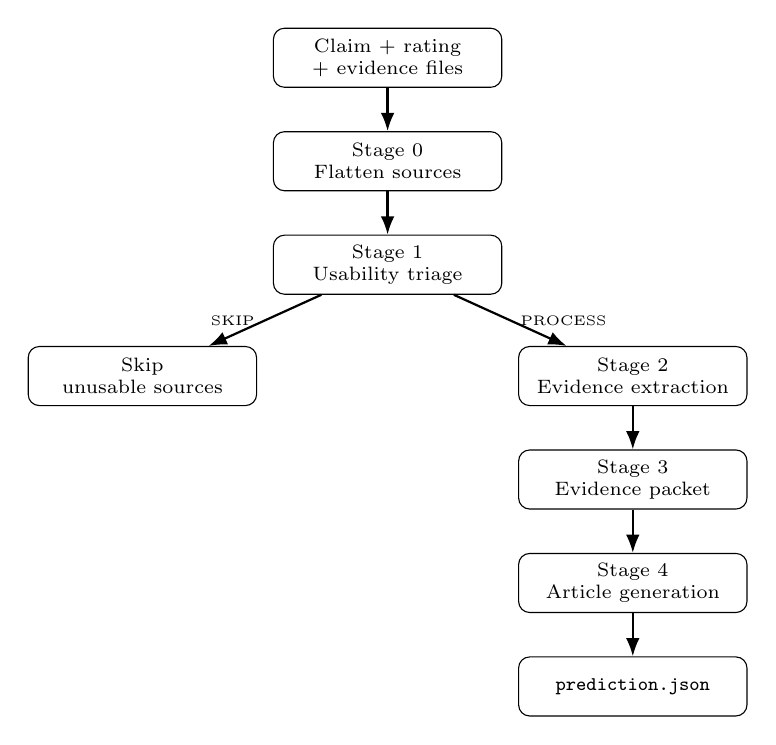
\begin{tikzpicture}[
    node distance=0.55cm and 0.9cm,
    box/.style={
        rectangle,
        rounded corners,
        draw,
        align=center,
        minimum width=2.9cm,
        minimum height=0.75cm,
        font=\scriptsize
    },
    arrow/.style={-Latex, thick}
]

\node[box] (data) {Claim + rating\\+ evidence files};
\node[box, below=of data] (stage0) {Stage 0\\Flatten sources};
\node[box, below=of stage0] (stage1) {Stage 1\\Usability triage};

\node[box, below left=0.65cm and 0.2cm of stage1] (skip) {Skip\\unusable sources};
\node[box, below right=0.65cm and 0.2cm of stage1] (stage2) {Stage 2\\Evidence extraction};

\node[box, below=of stage2] (stage3) {Stage 3\\Evidence packet};
\node[box, below=of stage3] (stage4) {Stage 4\\Article generation};
\node[box, below=of stage4] (pred) {\texttt{prediction.json}};

\draw[arrow] (data) -- (stage0);
\draw[arrow] (stage0) -- (stage1);
\draw[arrow] (stage1) -- node[left, font=\tiny]{SKIP} (skip);
\draw[arrow] (stage1) -- node[right, font=\tiny]{PROCESS} (stage2);
\draw[arrow] (stage2) -- (stage3);
\draw[arrow] (stage3) -- (stage4);
\draw[arrow] (stage4) -- (pred);

\end{tikzpicture}
\caption{Task 3 staged fact-checking article-generation pipeline.}
\label{fig:task3_pipeline}
\end{figure}

\section{Results and Discussion}

\subsection{Task 1: Source Retrieval for Scientific Web Claims}

To evaluate the evolution of our Task 1 system, we first report development-set results for the major retrieval, reranking, and fusion stages. These results were used for model selection and ablation analysis.

\begin{table*}[t]
  \caption{Task 1 development-set performance across major system stages.}
  \label{tab:task1_progression}
  \centering
  \begin{tabular}{lccccc}
    \toprule
    System & MRR@1 & MRR@5 & MRR@10 & Recall@5 & Recall@10 \\
    \midrule
    multilingual-e5-large retriever baseline & 0.5548 & 0.6282 & 0.6350 & 0.7416 & 0.7917 \\
    Qwen3-Embedding-8B LoRA retriever & 0.6147 & 0.6793 & 0.6876 & 0.7735 & 0.8348 \\
    Qwen3 retriever + BGE-reranker-v2-m3 & 0.6492 & 0.7094 & 0.7141 & 0.7996 & 0.8348 \\
    Qwen3 retriever + Nemotron reranker & 0.6742 & 0.7284 & 0.7323 & 0.8060 & 0.8348 \\
    Qwen3 retriever + Qwen3-Reranker-8B & 0.6956 & 0.7435 & 0.7466 & 0.8132 & 0.8348 \\
    Final three-model softmax fusion & \textbf{0.7146} & \textbf{0.7567} & \textbf{0.7594} & \textbf{0.8158} & 0.8348 \\
    \bottomrule
  \end{tabular}
\end{table*}

\begin{figure}[t]
  \centering
  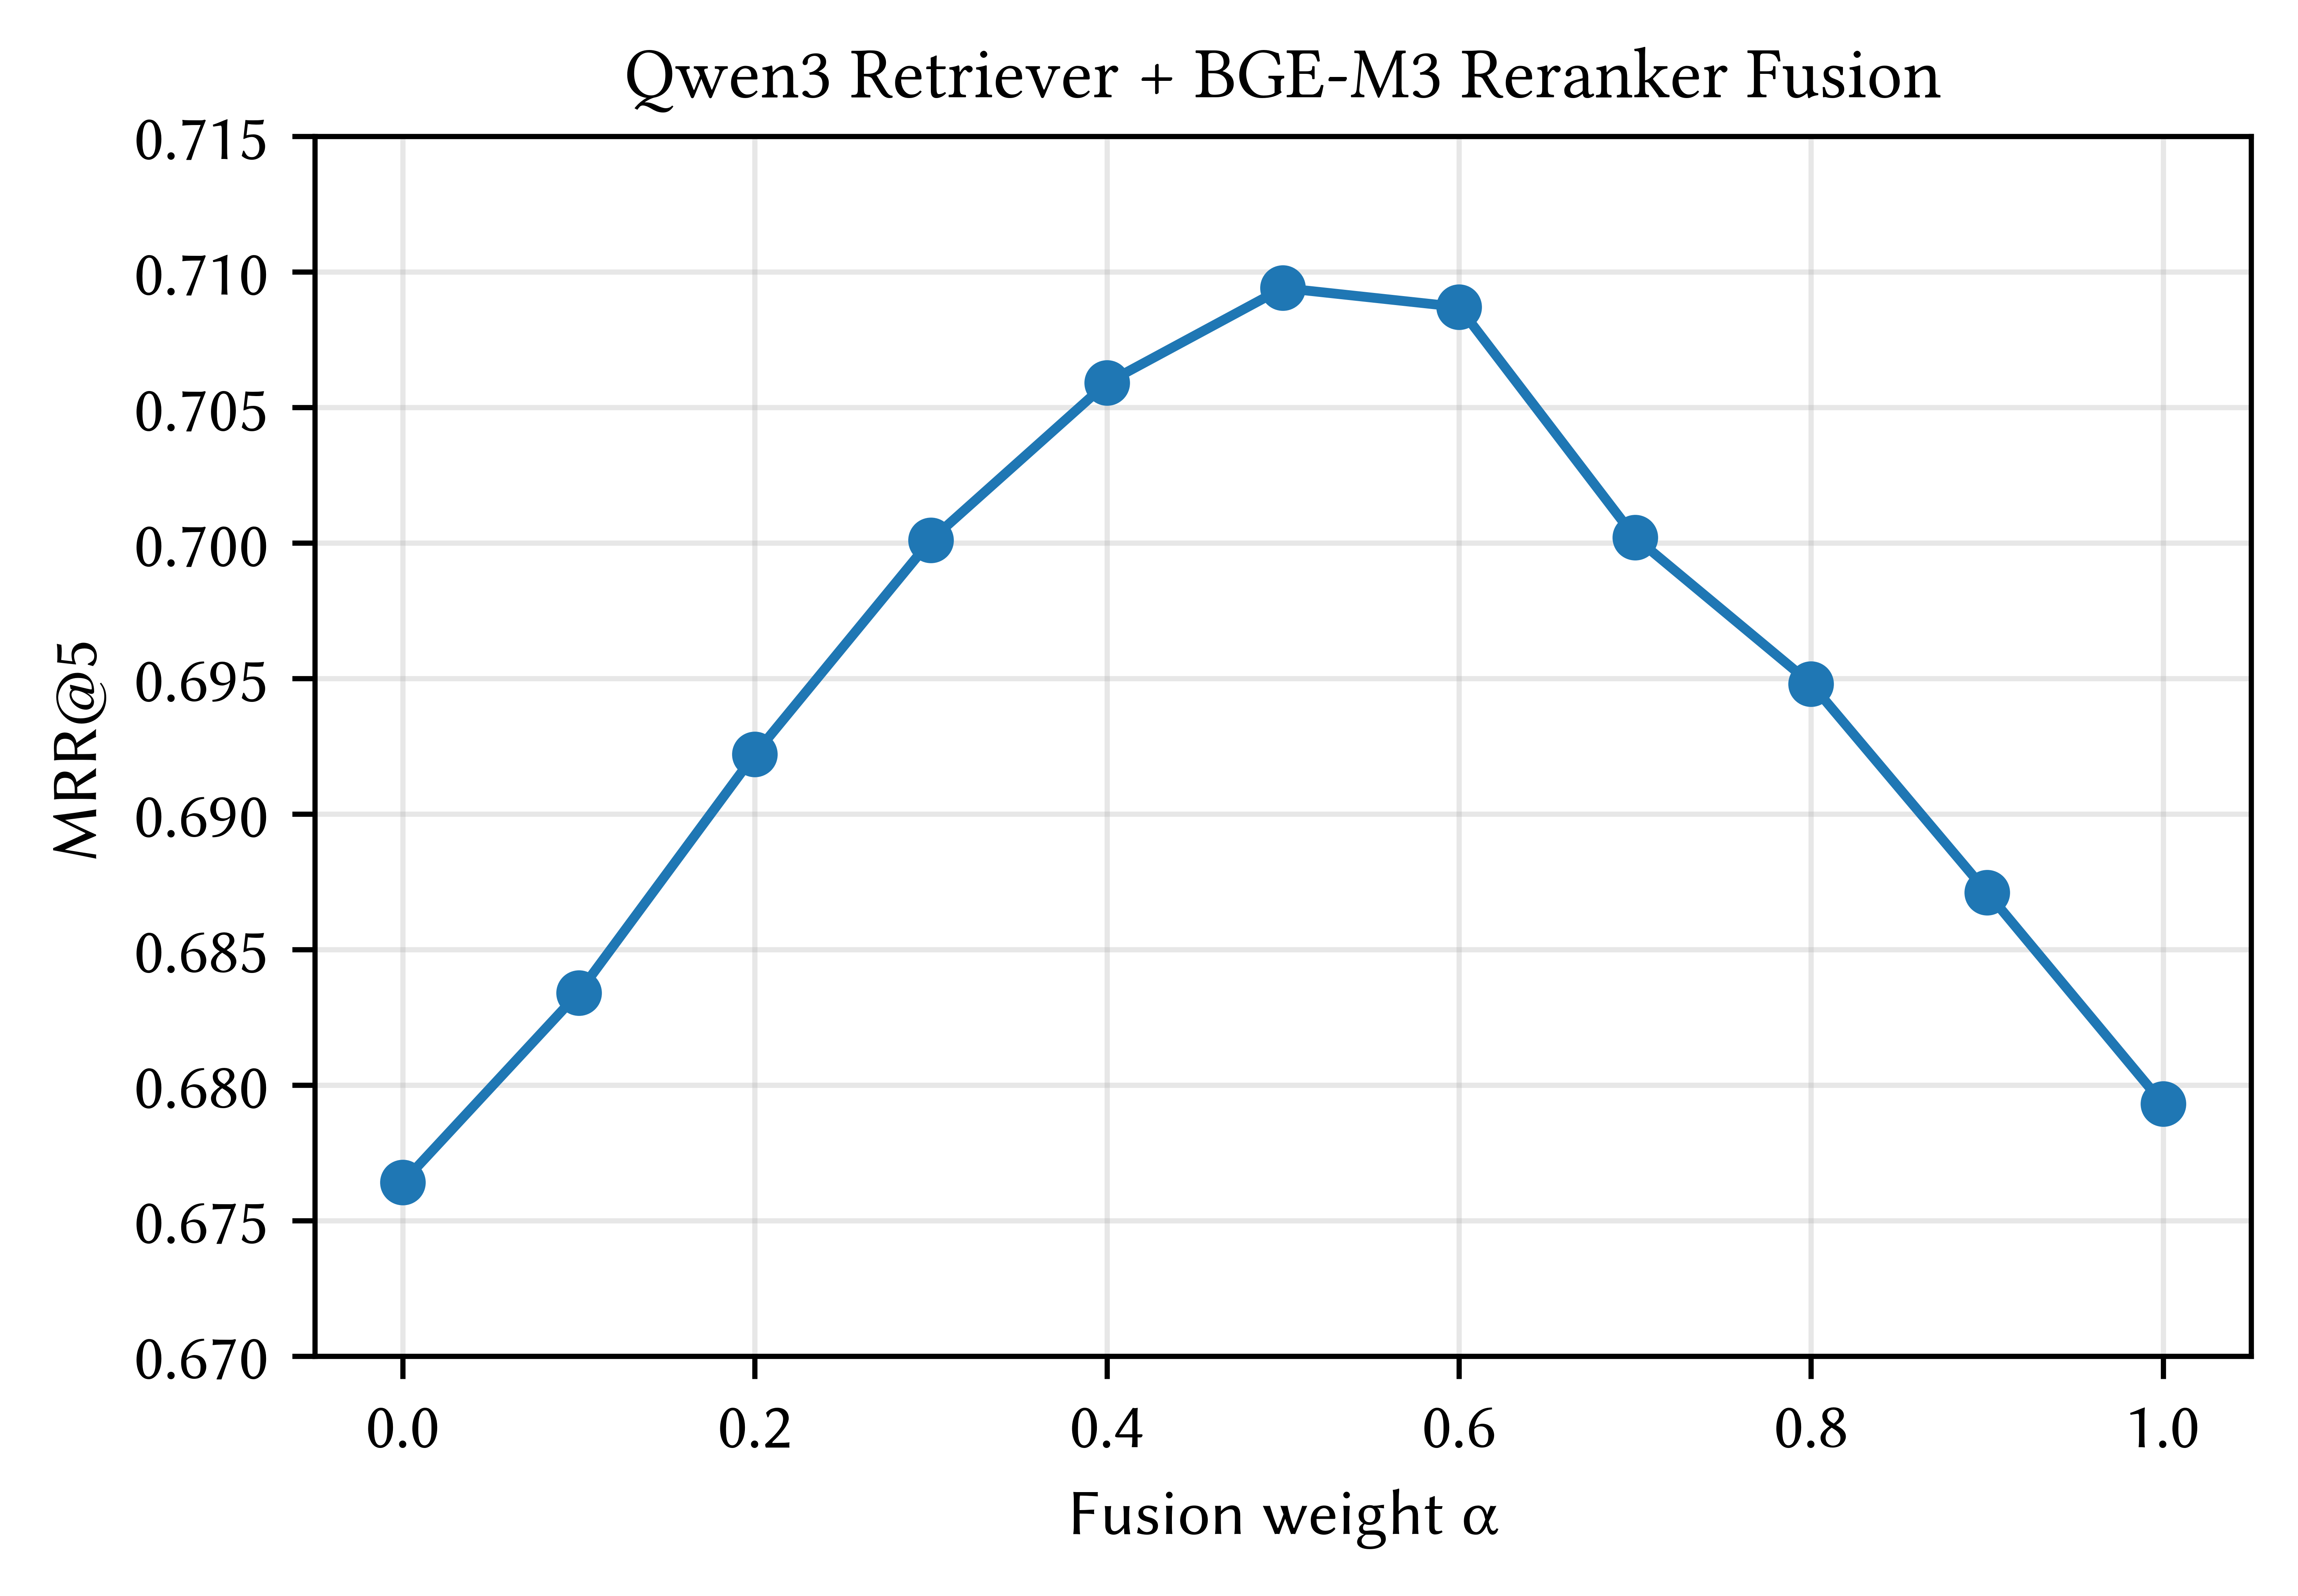
\includegraphics[width=0.65\linewidth]{task1_alpha_sweep.png}
  \caption{Development MRR@5 across dense/reranker fusion weights.}
  \label{fig:task1_alpha_sweep}
\end{figure}

Replacing \texttt{multilingual-e5-large} with LoRA-tuned Qwen3-Embedding-8B increased MRR@5 from 0.6282 to 0.6793, making candidate generation the largest early bottleneck.

We then trained task-specific listwise rerankers over the top-10 candidates retrieved by Qwen3-Embedding-8B. Figure~\ref{fig:task1_alpha_sweep} shows the first fusion experiment, where combining BGE-M3 reranker scores with Qwen3 retriever scores improved MRR@5 from 0.6764 for pure reranking and 0.6793 for pure retrieval to 0.7094 at $\alpha=0.5$. This result justified retaining fusion in later reranker experiments. Nemotron reached 0.7284 MRR@5 after fusion, while Qwen3-Reranker-8B was the strongest individual reranker, reaching 0.7435 MRR@5 after one epoch of LoRA training.

The final system combined the Qwen3 dense retriever, Qwen3-Reranker-8B, and Nemotron reranker using temperature-scaled softmax/log-probability fusion. To minimize variance and reduce the development-to-test generalization gap, we empirically tuned the fusion weights and temperatures via grid search on the development set. We found that language-specific configurations yielded the best results. For English, the optimal weights were $w_d=0.495$, $w_q=0.380$, and $w_n=0.125$, with temperatures $T_d=0.25$, $T_q=4.0$, and $T_n=4.0$. For French, the weights were $w_d=0.300$, $w_q=0.360$, and $w_n=0.340$ ($T_d=0.25, T_q=4.0, T_n=4.0$). For German, the weights were $w_d=0.475$, $w_q=0.355$, and $w_n=0.170$ ($T_d=0.25, T_q=4.0, T_n=3.0$). This optimized configuration achieved our peak development score of 0.7567 MRR@5, indicating that the rerankers provided complementary relevance signals rather than merely duplicating the retriever ranking.

\subsubsection{Ablation Findings}

Several ablations did not improve performance. Query cleaning and LLM-based style transfer sometimes removed useful lexical cues. German paraphrasing and back-translation gave no stable gain despite lower German data volume. Document chunking or hard-negative mining during the initial e5 retrieval stage was also not beneficial. Alternative retrievers, including BGE-M3, Harrier-OSS, and F2LLM-v2-14B, did not consistently outperform Qwen3-Embedding-8B, and zero-shot BGE reranking was weaker than task-trained reranking. Overall, the largest gains came from stronger candidate generation, listwise reranking on hard negatives, and calibrated score fusion.

We also submitted our final Task 1 system to Codabench under the team name \textit{CheckMate}. Table~\ref{tab:task1_codabench} reports our Codabench development and official evaluation-phase results.

\begin{table}[h]
  \caption{Codabench Task 1 results for team \textit{CheckMate}.}
  \label{tab:task1_codabench}
  \centering
  \begin{tabular}{lcccc}
    \toprule
    Phase & Avg. MRR@5 & DE & EN & FR \\
    \midrule
    Dev phase & 0.7600 & 0.7000 & 0.7600 & 0.8000 \\
    Evaluation/Test phase & 0.7194 & 0.6861 & 0.7343 & 0.7378 \\
    \bottomrule
  \end{tabular}
\end{table}

The Codabench development-phase result of 0.7600 average MRR@5 is consistent with our internal development result of 0.7567 MRR@5 after rounding. However, the official evaluation-phase score dropped to 0.7194 average MRR@5. This indicates that the final fusion strategy generalized reasonably but was still tuned heavily on the development split. The largest drop occurred in French, where the development score was 0.8000 but the evaluation score was 0.7378. German remained the most difficult language in both phases, with 0.7000 MRR@5 on the development phase and 0.6861 on the evaluation phase.

\begin{table}[h]
  \caption{Official Codabench evaluation-phase leaderboard excerpt for Task 1.}
  \label{tab:task1_leaderboard}
  \centering
  \begin{tabular}{lcccc}
    \toprule
    Team & Avg. MRR@5 & DE & EN & FR \\
    \midrule
    claim2source & 0.7628 & 0.7153 & 0.7819 & 0.7912 \\
    team-outsider & 0.7580 & 0.7228 & 0.7802 & 0.7709 \\
    mattiaskvist & 0.7464 & 0.7070 & 0.7571 & 0.7752 \\
    CheckMate & 0.7194 & 0.6861 & 0.7343 & 0.7378 \\
    \bottomrule
  \end{tabular}
\end{table}

Although our development score was competitive, the evaluation-phase leaderboard shows a larger generalization gap for our final system compared with the top submissions. This suggests that future work should tune fusion parameters using more robust validation strategies, such as cross-validation or held-out language-specific calibration splits, rather than relying heavily on the public development set.

\subsection{Task 2: Fact-Checking Numerical Claims}

The evaluation metrics of interest for Task 2 are macro F1 and Recall@5. Recall@5 measures the quality of the ranked reasoning traces, while macro F1 measures final claim-verification performance.

Table~\ref{tab:task2_results} reports validation results across the baseline, parameter-scaling, pairwise-ranking, PRP, PREPAIR, and DPO+BT approaches.

In the English subset, the transition from the 1B baseline to the quantized 3B model yielded the most substantial performance gains. We observe a 15\% relative increase in Macro-F1 and a modest improvement in ranking utility (Recall@5). Whereas a comparison between the Pointwise 1B baseline and the Pairwise 1B model reveals that the Pairwise model improved the Macro-F1 by 9\% over the baseline.  However, interestingly, the Pairwise model showed degradation in Recall@5 (0.3010 $\to$ 0.2757). This drop suggests that the tournament approach is superior at identifying the single best trace (improving F1), but the aggregated win-scores probably introduce slight noise in the lower ranks compared to absolute pointwise scoring.

Pairwise Ranking Prompting (PRP) successfully recovers some of the lost ranking utility in English, raising Recall@5 to 0.2835 and further boosting the Macro-F1 to 0.5170. This underscores the importance of debiasing techniques when using small-parameter models for relational reasoning.

The PREPAIR approach achieved the highest Macro-F1 among the 1B models in both English (0.5194) and Arabic (0.5297). By injecting scorecards derived from the pointwise model into the pairwise prompt, PREPAIR provides a cognitive anchor that helps the model avoid context collapse. However, this comes at the cost of lower sensitivity to the top-five ranking distribution, as reflected by the decline in English Recall@5 to 0.2695.

In contrast, the DPO + Bradley-Terry (BT) approach yielded mixed results. While it underperformed in English, it proved remarkably effective for the Spanish subset, achieving the highest Macro-F1 (0.4049) and Recall@5 (0.2574) for that language. This could indicate that the Bradley-Terry framework offers a stable, transitive ranking signal on smaller, more focused datasets where dense pairwise tournaments might lead to overfitting.

Lastly, the Arabic subset highlights a distinct performance gap. While PrePAIR boosts classification accuracy significantly (0.5297), no pairwise or advanced ranking approach is able to beat the simple 1B Pointwise baseline in Recall@5 (0.2786). A hypothesis for this is that Arabic has increased token density and structural complexity for pairwise comparison, which essentially doubles the prompt length and may exceed the reasoning density, degrading the output quality.

The table below shows the results obtained on the validation dataset:

\begin{table}[ht]
\centering
\caption{Comparative Performance Across Languages and Model Architectures.}
\label{tab:task2_results}
\begin{tabular}{llcccccc}
\toprule
\textbf{Language} & \textbf{Metric} & \textbf{Baseline} & \textbf{Llama 3.2 3B} & \textbf{Pairwise} & \textbf{PRP} & \textbf{PREPAIR} & \textbf{DPO + BT}\\
\midrule
\multirow{2}{*}{English} & Macro-F1 & 0.4628 & 0.5324 & 0.5061 & 0.5170 & \textbf{0.5194} & 0.4936\\
& Recall@5 & 0.3010 & 0.3129 & 0.2757 & 0.2835 & 0.2695 & 0.2659\\
\midrule
\multirow{2}{*}{Arabic}  & Macro-F1 & 0.4917 & --- & 0.5210 & 0.3555 & \textbf{0.5297} & 0.5172 \\
& Recall@5 & \textbf{0.2786} & --- & 0.2400 & 0.2349 & 0.2466 & 0.2485 \\
\midrule
\multirow{2}{*}{Spanish} & Macro-F1 & 0.3654 & --- & 0.3804 & 0.3807 & 0.4003 & \textbf{0.4049} \\
& Recall@5 & 0.2401 & --- & 0.2425 & 0.2422 & 0.2090 & \textbf{0.2574} \\
\bottomrule
\end{tabular}
\end{table}

Due to last-minute submission issues, only the Arabic and Spanish runs were officially submitted on Codabench; the English result is reported as an internal project result.

\begin{table}[h]
  \caption{Task 2 results. Arabic and Spanish are official Codabench test results; English is reported as an internal result.}
  \label{tab:task2_codabench}
  \centering
  \begin{tabular}{lcccc}
    \toprule
    Language & Rank & Avg Score & Macro-F1 & Recall@5\\
    \midrule
    Spanish & 9th & 0.4093 &  0.5662 & 0.2525\\
    Arabic & 11th & 0.5599 & 0.8407 &  0.2792\\
    English (internal) & N/A & 0.4115 & 0.2320 & 0.5909\\
    \bottomrule
  \end{tabular}
\end{table}

\subsection{Task 3: Generating Full Fact-Checking Articles}

Table~\ref{tab:task3_codabench} reports the official Task 3 results for our final submission. The system achieved an overall mean score of 0.328, with stronger citation precision, citation recall, and evidence coverage than entailment. This suggests that deterministic citation control helped maintain valid source use, but the generated sentences were not always tightly supported by the cited evidence.

\begin{table}[h]
  \caption{Official Task 3 Codabench scores for team \textit{CheckMate}.}
  \label{tab:task3_codabench}
  \centering
  \begin{tabular}{lc}
    \toprule
    Metric & Score \\
    \midrule
    Mean entailment score & 0.221 \\
    Mean citation precision & 0.350 \\
    Mean citation recall & 0.350 \\
    Mean evidence coverage & 0.391 \\
    Overall mean score & 0.328 \\
    \bottomrule
  \end{tabular}
\end{table}

Internal diagnostics suggest that the pipeline applied conservative source-use decisions before article generation. Of 8,979 flattened source-level records, 5,741 were passed forward as \texttt{PROCESS}, while 3,238 were filtered out at the usability-triage stage. After repaired Stage 2 extraction, sources were distributed across \texttt{useful\_context} (2,251), \texttt{direct\_evidence} (2,103), \texttt{off\_topic} (986), \texttt{claim\_origin} (939), and \texttt{no\_content} (282). Rather than treating all evidence uniformly, the system attempted to distinguish direct verification evidence from contextual or claim-origin material. This made the generation process safer, but may also have limited the amount of evidence available for broader coverage and stronger sentence-level entailment.

Stage 4 validation reflects the same precision-oriented design. The initial article set contained 96 validation-error rows and 156 zero-citation rows. A deterministic post-generation rescue pass reduced validation errors to zero and reduced zero-citation rows to 33, while preserving the required output structure. However, the official scores show that structural validity and citation control did not fully translate into strong entailment performance. This suggests that future versions should relax evidence-use decisions more carefully, while adding sentence-level entailment checks to ensure that generated claims remain closely supported by their citations.

\section{Conclusion}

This paper presented our participation as team \textit{CheckMate} in the CheckThat! 2026 Lab across three tasks.

For Task 1, the strongest gains came from replacing the initial dense retriever with Qwen3-Embedding-8B, adding task-trained reranking, and applying calibrated multi-model fusion; the final system achieved 0.7194 average MRR@5 on the official evaluation phase.

For Task 2, we found that both model scale and ranking methodology affected numerical claim verification. Moving from the 1B pointwise baseline to a quantized 3B model produced the strongest English-language gain. Pairwise methods improved final verdict prediction in several settings, but sometimes reduced Recall@5, suggesting that identifying the single best trace and preserving a strong top-five ranking are not always aligned. PREPAIR performed strongly in English and Arabic by adding structured scorecard information before comparison, while DPO with Bradley-Terry reward modeling was most effective for Spanish. Future work could explore reinforcement-learning-based ranking strategies such as Iterative Exclusion Ranker, where the model learns to eliminate weaker candidates step by step rather than scoring all traces independently \cite{IRRanker}. With greater computational resources, full round-robin pairwise tournaments could also be revisited, since they may provide richer comparison signals than the more efficient elimination-based setup used in our experiments.

For Task 3, we built a staged LLM-assisted article-generation pipeline with conservative evidence selection, deterministic citation insertion, and post-generation validation. The final submission achieved an overall mean score of 0.328, with zero validation-error rows after rescue. However, the lower entailment score shows that valid citation formatting alone is insufficient; future work should better balance citation control, evidence coverage, and sentence-level support.

Across all three tasks, our results suggest that decomposed fact-checking pipelines are useful because retrieval, reasoning-trace ranking, evidence selection, and article generation introduce different failure modes. Future work should focus on stronger validation strategies, multilingual calibration, and tighter integration between citation-aware generation and entailment-based checking.

\section*{Declaration on Generative AI}
During the preparation of this work, the authors used Generative AI tools including Gemini and NotebookLM to support literature survey exploration and drafting assistance. The authors manually reviewed, edited, and verified the resulting content. In addition, Gemini models were used as part of the implemented Task 3 system for source usability triage, claim-aware evidence extraction, and fact-checking article generation. The authors take full responsibility for the paper's content and submitted system outputs.

%%
%% Define the bibliography file to be used
\bibliography{sample-ceur}

%%
%% If your work has an appendix, this is the place to put it.
% \appendix

% \section{Online Resources}


% The sources for the ceur-art style are available via
% \begin{itemize}
% \item \href{https://github.com/yamadharma/ceurart}{GitHub},
% % \item \href{https://www.overleaf.com/project/5e76702c4acae70001d3bc87}{Overleaf},
% \item
%   \href{https://www.overleaf.com/latex/templates/template-for-submissions-to-ceur-workshop-proceedings-ceur-ws-dot-org/pkfscdkgkhcq}{Overleaf
%     template}.
% \end{itemize}

\end{document}

%%
%% End of file

